\documentclass[a4paper,11pt,hidelinks]{article}
%\usepackage[a-1b]{pdfx}
\usepackage{hyperref}

\usepackage{subfiles}
\usepackage{epsfig}
\usepackage{plain}
\usepackage{setspace}
%\usepackage{minted}
\usepackage{listings}

\usepackage{mdframed}
\usepackage{caption}
\usepackage{color}
\usepackage{amsmath}
\usepackage{amsthm}
\usepackage{amssymb}
\usepackage{amsfonts}
\usepackage{mathabx}
\usepackage{tcolorbox}
\usepackage{multicol}
\usepackage[english]{babel}
\usepackage[left=2cm,right=2cm,top=2cm,bottom=1.8cm]{geometry}
\usepackage{titlesec} 
\usepackage[utf8x]{inputenc} 

\hypersetup{colorlinks=true, urlcolor=blue}

\captionsetup{
  justification=centering,
  singlelinecheck=false,
  font=small,labelfont=bf,labelsep=space}

\begin{document}

\pagestyle{plain}

\begingroup

\renewcommand{\cleardoublepage}{}
\renewcommand{\clearpage}{}

\titleformat{\section}
{\normalfont\Large\bfseries}{\thesection}{1em}{}


\renewcommand{\lstlistingname}{Code}%
\renewcommand{\lstlistlistingname}{List of \lstlistingname s}

\definecolor{codeBackground}{rgb}{0.9, 0.9, 0.9}

% Code environment
\lstnewenvironment{code}[1]{
  \mdframed[%
    backgroundcolor=codeBackground,
    shadow=false,
    linecolor=black!40,
    linewidth=2pt,
    topline=false,
    rightline=false,
    leftline=false
  ]%
  \lstset{%
    moredelim=**[is][\color{blue}]{**}{**},
    moredelim=**[is][\color{teal}]{.-}{-.},
    moredelim=**[is][\color{gray}]{||}{||},
    frame=single,
    framerule=0pt,
    basicstyle=\ttfamily,
    columns=fullflexible
  }%
}{% Spacing between and after caption + before end of mdframed
  \vspace{-1em}
  \endmdframed
  \vspace{-0.5em}
  \captionsetup{type=lstlisting}
  \caption{#1}
  \vspace{1.5em}
  \ignorespaces
}

\newpage

\title{SYN flood exercise}
\author{Offensive Technologies 2021 \\
  Matteo Franzil \texttt{<matteo.franzil@studenti.unitn.it>}}
\maketitle

\section{Solution}

This instruction file solely contains the information needed for replicating the experiment. In order to see the answers to the required questions, please see the \verb=memo.pdf= file.

\subsection{Setting up}

In order to get started, i first opened a four-panel terminal session, one for each node in the experiment. This made easier the data collection later on.

\begin{figure}[h!]
  \centering
  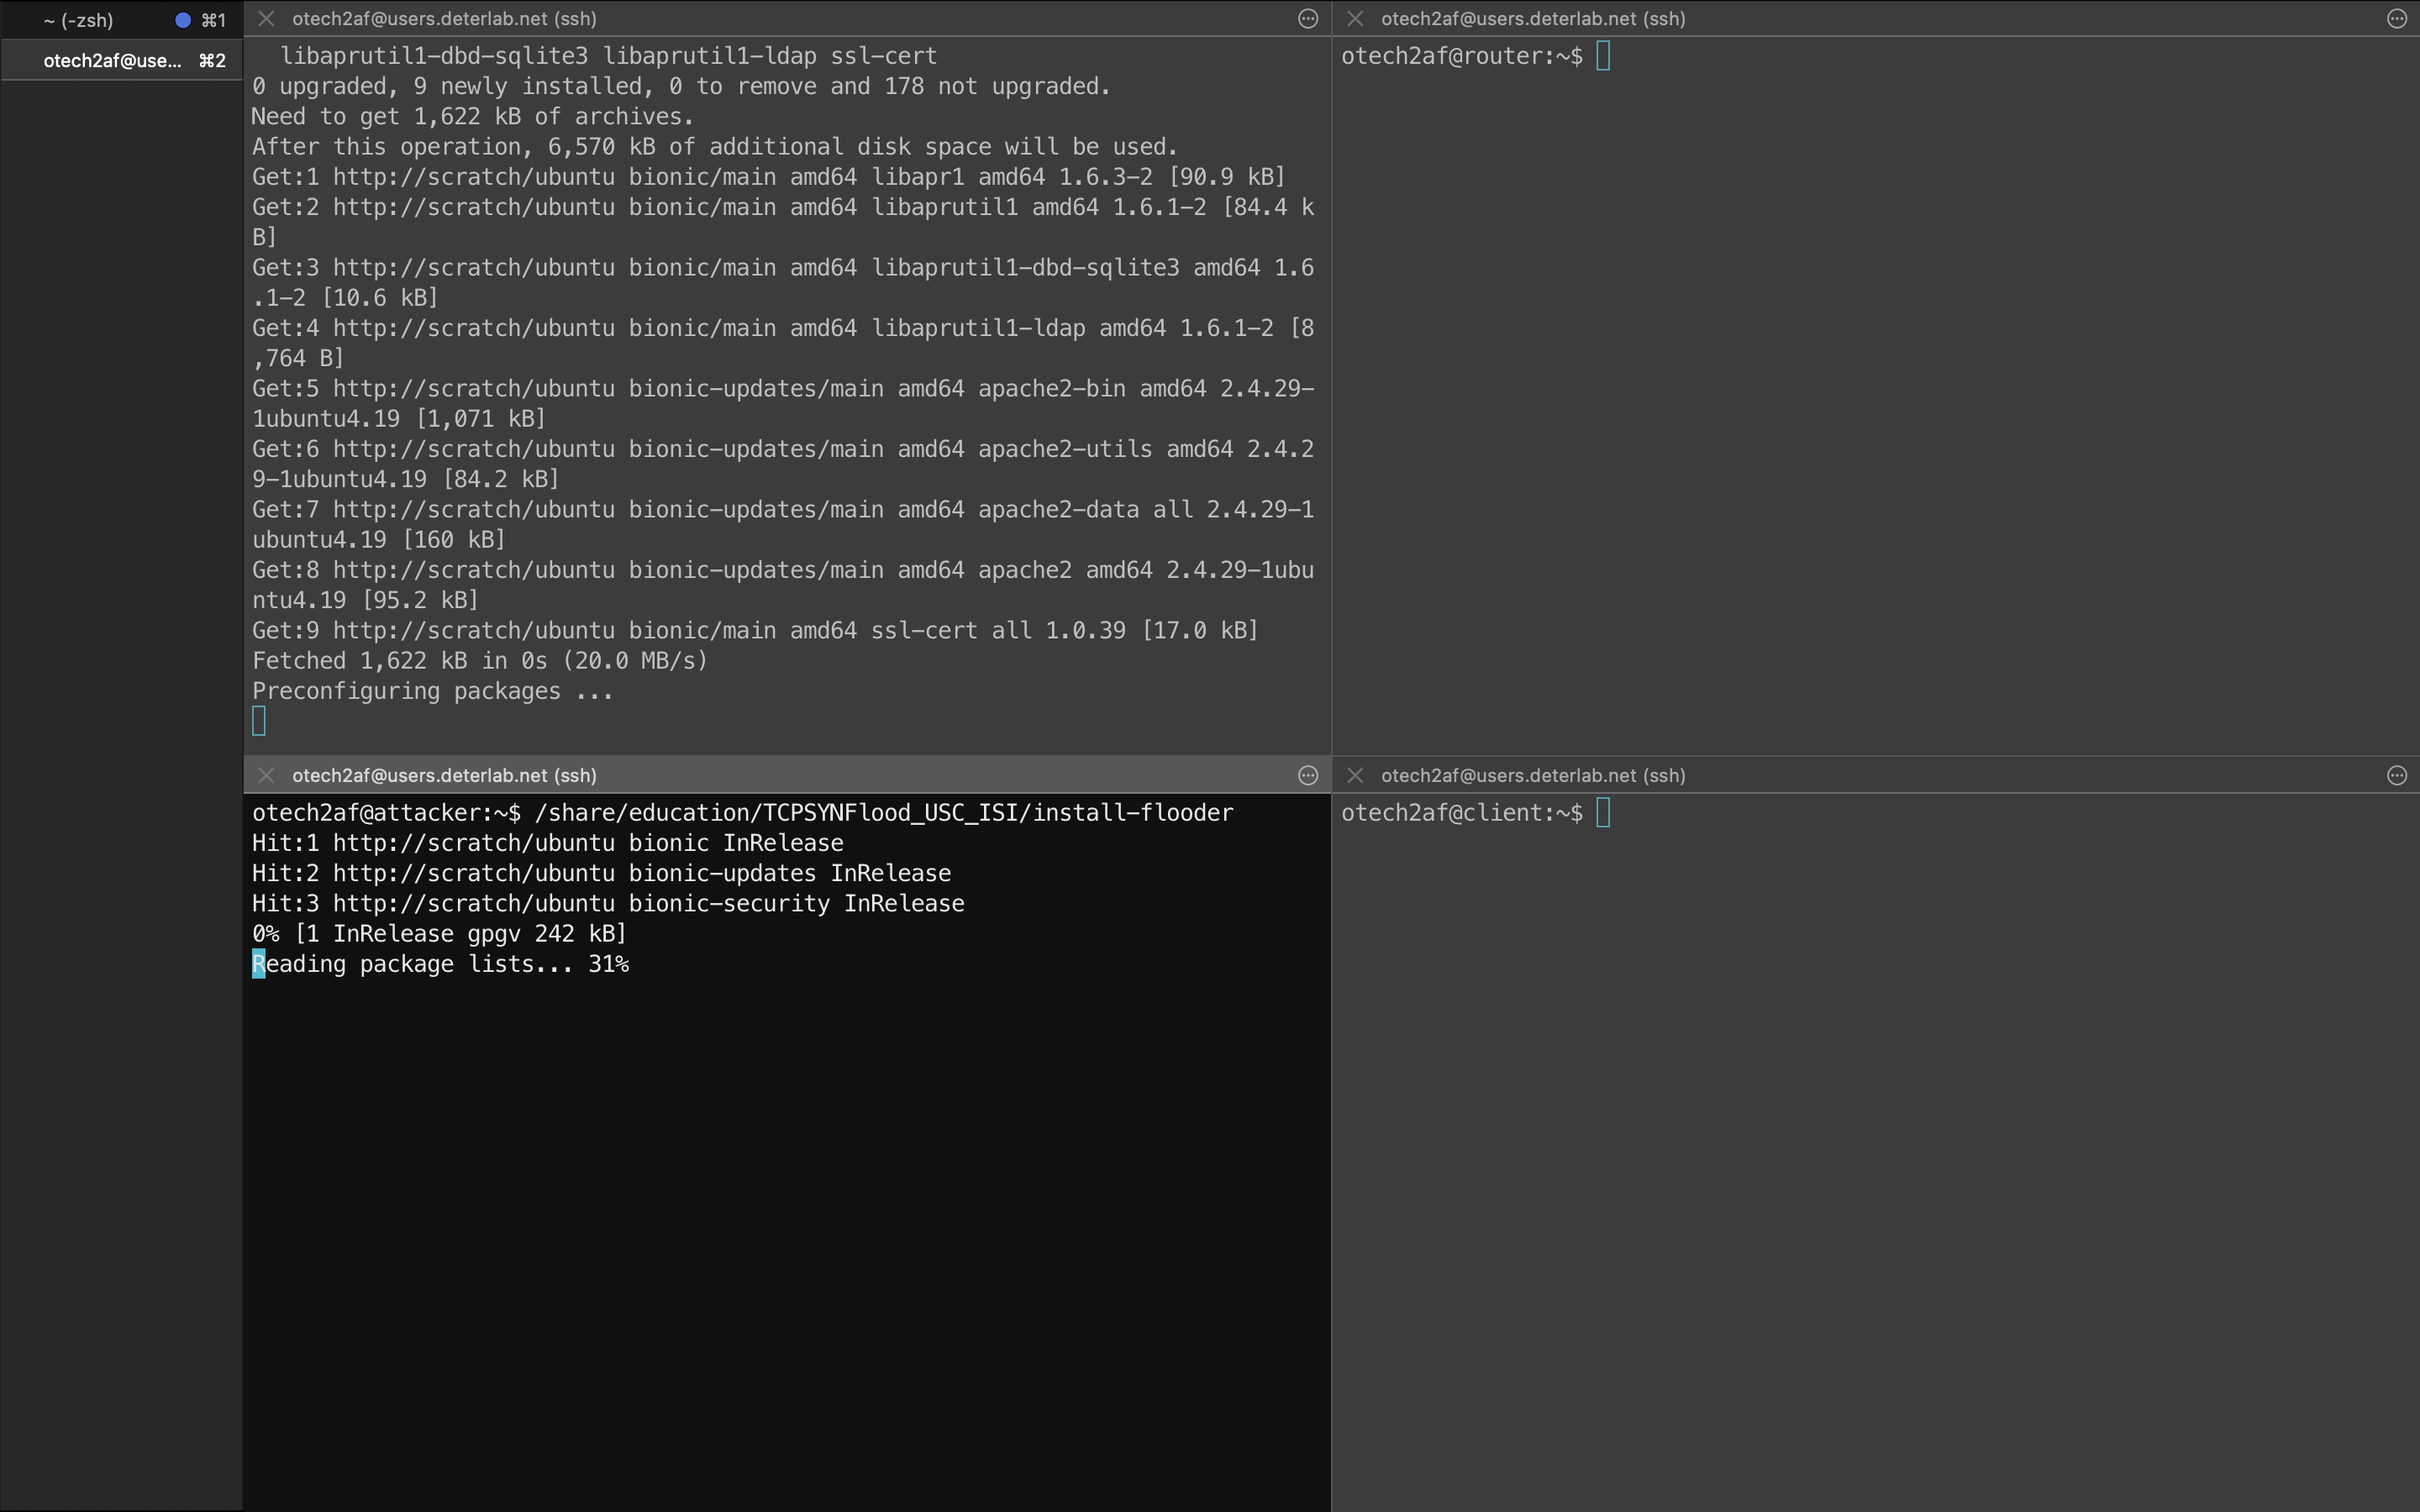
\includegraphics[width=0.8\textwidth]{../drawable/setup.png}
  \caption{Setting up our environment.}
\end{figure}

For each of the nodes - bar the \verb=router=, which I seldom used and only for quick \verb=tcpdump= visits - I ran the following scripts, in order to set them up and later start the SYN flooding (or regular requests, for the client). For the client, I chose to keep \verb=tcpdump= on the background in order to have focus on the script making requests, which could be then easily terminated with \verb=^C=.

I decided to settle on \verb=1000= packets per second for the DoS attack, a good compromise between crashing the webserver and having statistically insignificant results.

\begin{code}{Code for the client}
  cat <<EOF > script.sh
  #!/bin/bash
  while sleep 1; do curl server/index.html >/dev/null 2>/dev/null; done;
  EOF

  # sudo tcpdump -nn -i eth1

  chmod +x script.sh
  sudo tcpdump -nn -v -s0 -i ${ETH} -w cookie.pcap &
  ./script.sh
\end{code}

\begin{code}{Code for the attacker}
  /share/education/TCPSYNFlood_USC_ISI/install-flooder

  sudo flooder --dst 5.6.7.8 --src 1.1.2.0
  --srcmask 255.255.255.0 --highrate 100
  --lowrate 100 --proto 6 --dportmin 80
  --dportmax 80
\end{code}

\begin{code}{Code for the server}
  SYNCOOKIES=$(sudo sysctl net.ipv4.tcp_syncookies | awk '{print $3}')
  if [[ $SYNCOOKIES -eq 1 ]]; then
  sudo sysctl -w net.ipv4.tcp_syncookies=0
  sudo sysctl -w net.ipv4.tcp_max_syn_backlog=10000
  fi
  SYNCOOKIES=$(sudo sysctl net.ipv4.tcp_syncookies | awk '{print $3}')
  if [[ $SYNCOOKIES -eq 0 ]]; then echo "OK"; else echo "KO"; fi

  /share/education/TCPSYNFlood_USC_ISI/install-server

  sudo tcpdump ip -i ${ETH}
\end{code}

\subsection{Gathering data}

I gathered data for the following different setups:

\begin{itemize}
  \item \verb=REQ1=: syn-cookies: \textbf{on}, spoofing: \textbf{on}, network setup: \textbf{1};
  \item \verb=REQ2=: syn-cookies: \textbf{off}, spoofing: \textbf{on}, network setup: \textbf{1};
  \item \verb=EXT1=: syn-cookies: \textbf{off}, spoofing: \textbf{off}, network setup: \textbf{1} (extra point 1); 
  \item \verb=EXT2=: syn-cookies: \textbf{off}, spoofing: \textbf{off}, network setup: \textbf{2} (extra point 2);
\end{itemize}

\begin{figure}[h!]
  \centering
  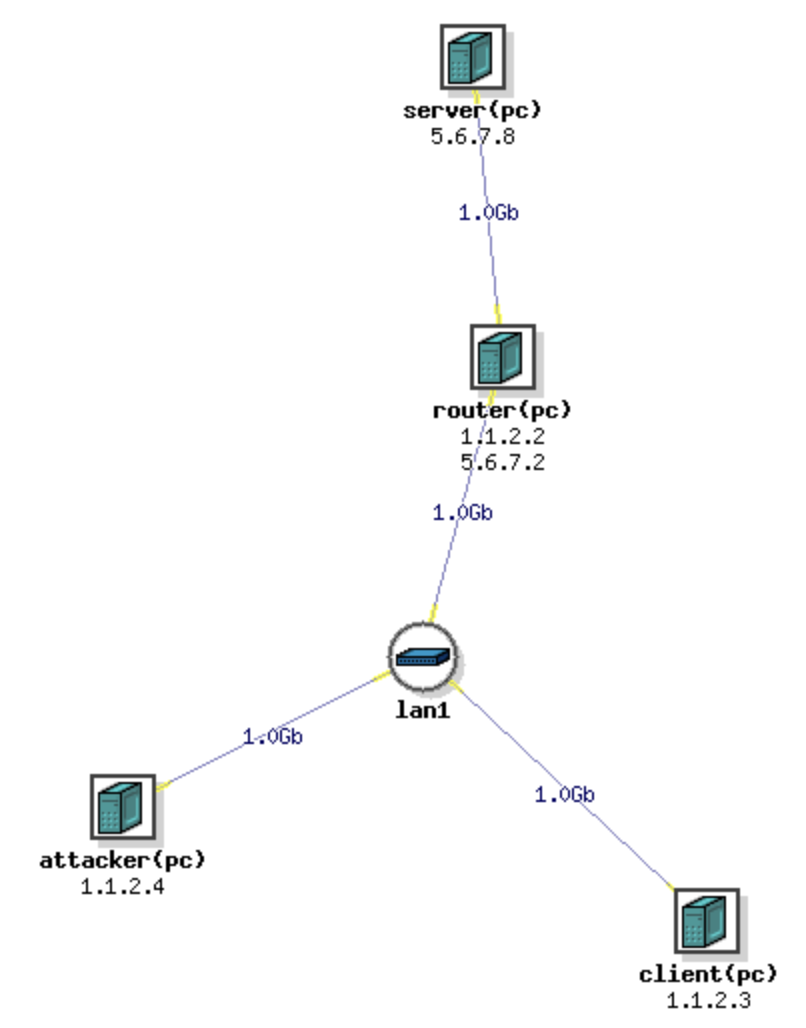
\includegraphics[width=0.44\textwidth]{../drawable/network.png}
  \caption{Network used for the first three setups.}
\end{figure}

\begin{figure}[h!]
  \centering
  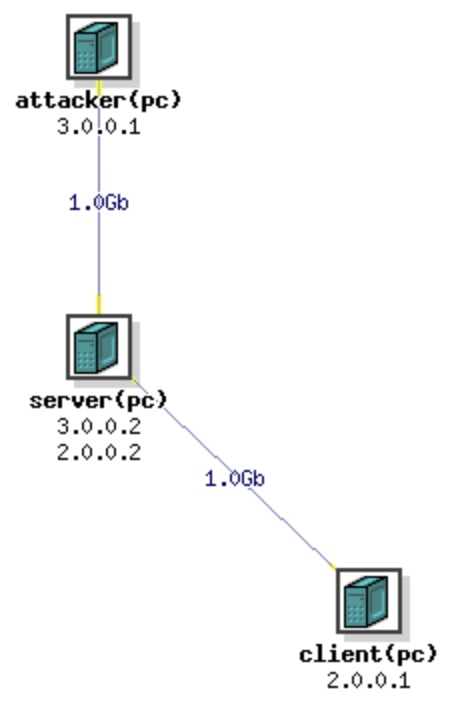
\includegraphics[width=0.25\textwidth]{../drawable/network-extra2.png}
  \caption{Network used for the last setup.}
\end{figure}


Each setup was run with the following schedule (measured with a timer on my smartphone), for a total of 180 seconds each:

\begin{enumerate}
  \item 30 seconds of client-only traffic;
  \item 120 seconds of both attacker and client traffic;
  \item 30 more seconds of client-only traffic.
\end{enumerate}

This data was written in the \verb=cookie.pcap= file, \verb=scp=ied it to my PC, and opened with Wireshark. Then, it was further filtered and inspected (by removing runaway packets and observing the position of eventual ICMP error messages), and viewed with the Conversation view - which allows you to visualize the packets in a compact form, in which TCP sessions are condensed into a single line. Code 4 shows an example of a visualization provided by Wireshark:

\begin{code}{Sample line (split in two) and key from the Wireshark conversation panel}
  Address A----Port A----Address B---Port B----Packets---Bytes
  1.1.2.3------58250-----5.6.7.8-----80--------14--------12193

  Pk A>B---Bytes A>B---Pk B>A---Bytes B>A---Rel Start-----Duration
  8--------616---------6--------11577-------1,031706------0,002221
\end{code}

For each of the setups, I exported the visualization for the whole 180 seconds of the setup to CSV and processed the data with Excel.

In the following tables, the \textit{average duration} field refers to the total duration of the TCP session from the first \verb=SYN= to the last packet (\verb=RST/SYN=). As requested, timed out connections are assigned a duration of \verb=200= seconds.

\subsubsection{\texttt{REQ1} results}

With this setup - syn-cookies on - we can see that the traffic kept flowing as expected, with connection duration only receiving a very small increase. This difference is amplified by the small scale of the graph, but still lies in the milliseconds and does not impact legitimate traffic at all.

\begin{figure}[h!]
  \centering
  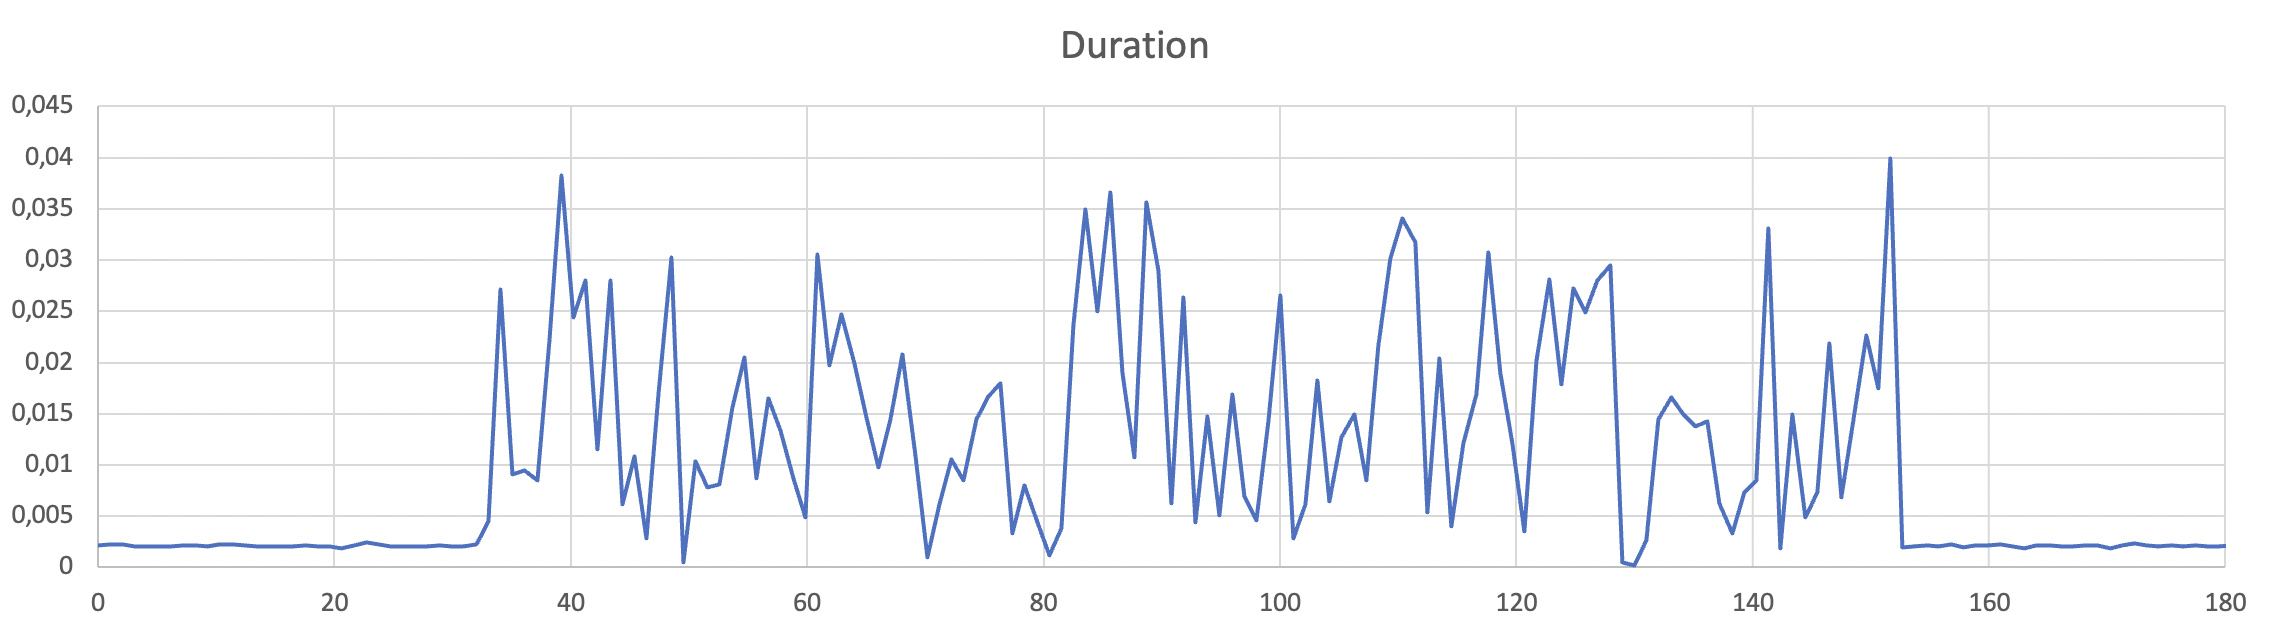
\includegraphics[width=0.8\textwidth]{../drawable/req1.png}
\end{figure}

\begin{table}[h!]
  \centering
  \begin{tabular}{|l|l|}
    \hline
    Traffic         & Average duration (s)    \\ \hline
    regular traffic & \verb=0.002105= \\ \hline
    with DoS        & \verb=0,147= \\ \hline
    overall         & \verb=0.01072= \\ \hline
  \end{tabular}
\end{table}

\subsubsection{\texttt{REQ2} results}

In this setup - without syn-cookies - we can see that unlike in \verb=REQ1=, during the DoS attack we have a complete loss of traffic. Indeed, during the 120-second window I recorded a single, clean packet originating from the client (which never received a reply), while I recorded \verb=15= additional spoofed response packets, originating from the server. These packets were generated as a result of the spoofed attacker's request, and the client promptly replied with a \verb=RST= - as the receiving port was not of course open.

I tried to tune down the amount of packets per second to 500, 300 and less, and I started having a rebound in traffic (i.e. some lucky session managing to close in 30 seconds or less) starting from 250 packets per second. Still, such numbers are irrealistic and too low for a proper DoS attack, even the weakest one.

The graphic (and subsequent ones) has a logarithmic y-axis to account for the extreme difference between small fluctuations in the regular traffic (in milliseconds) and slowed down traffic (in seconds)

\begin{figure}[h!]
  \centering
  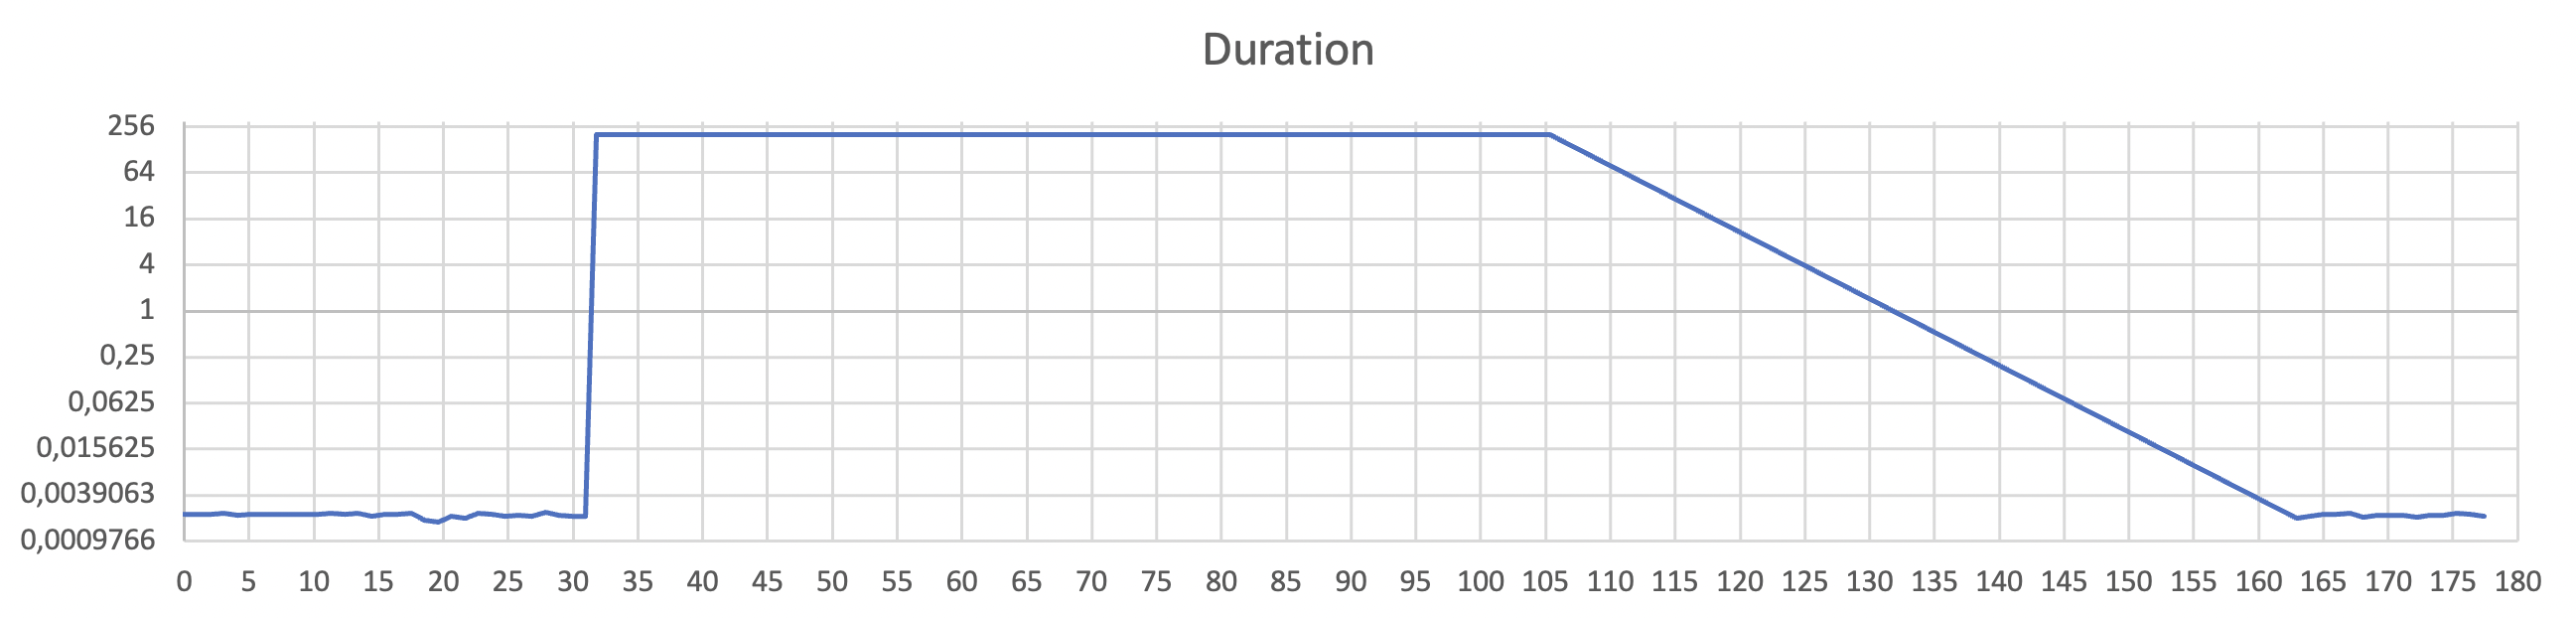
\includegraphics[width=0.8\textwidth]{../drawable/req2.png}
\end{figure}

\begin{table}[h!]
  \centering
  \begin{tabular}{|l|l|}
    \hline
    Traffic         & Average duration (s)    \\ \hline
    regular traffic & \verb=0.002138= \\ \hline
    with DoS        & \verb=200= \\ \hline
    overall         & \verb=19.60= \\ \hline
  \end{tabular}
\end{table}

\newpage

\subsubsection{\texttt{EXT1} results}

With this setup - syn-cookies off and spoofing off - we obtained similar result to \verb=REQ2=, with the single difference that we obtained a single packet with a duration of 200 seconds. This happened since we deactivated spoofing, and so the attacker was no longer crafting packets whose response would be directed back at the client.

\begin{figure}[h!]
  \centering
  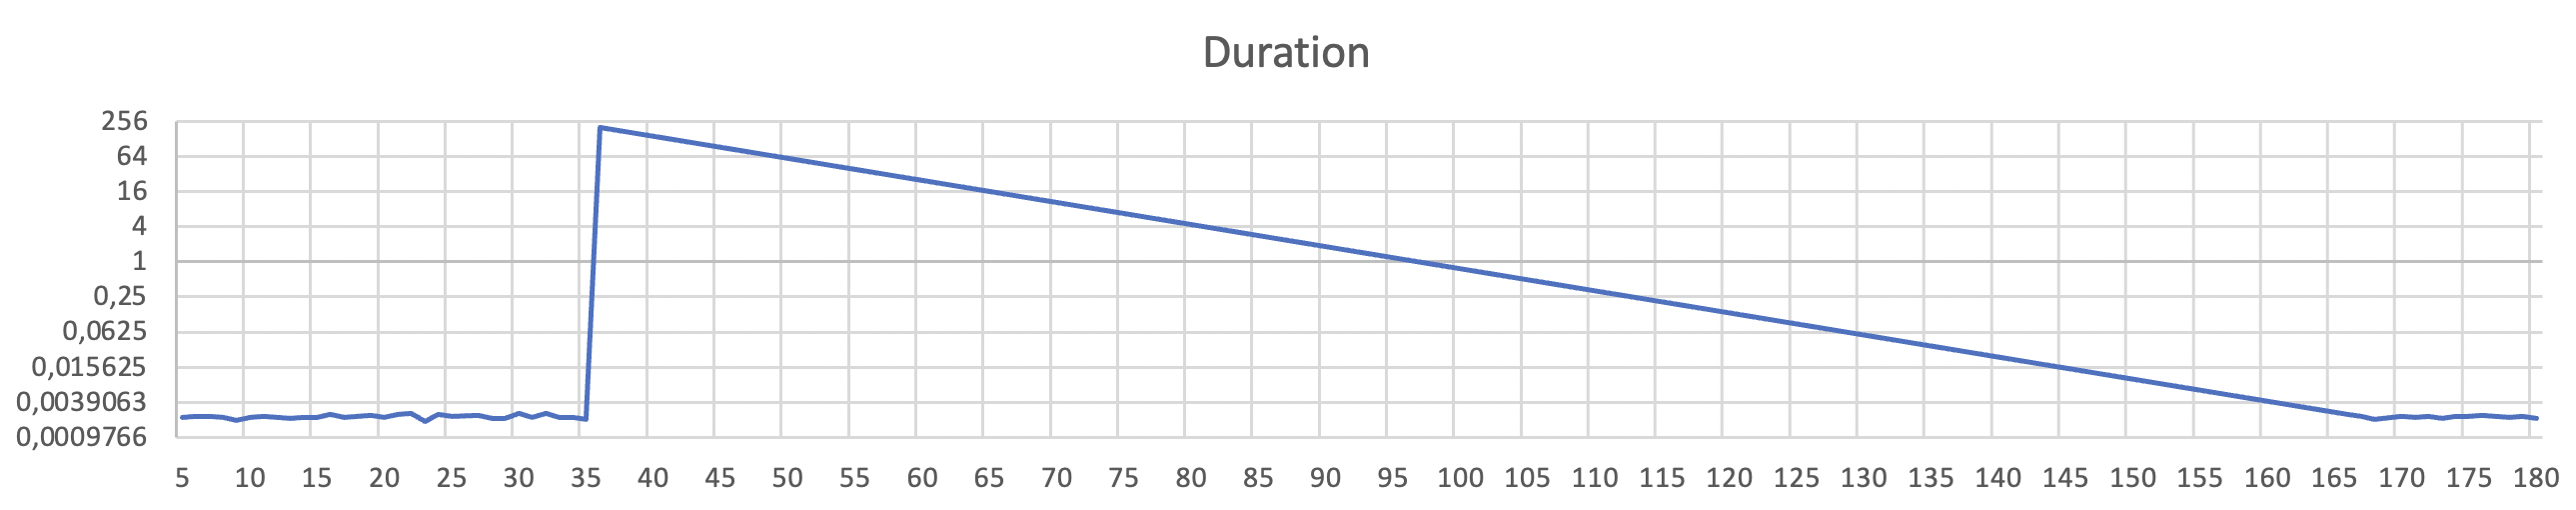
\includegraphics[width=0.8\textwidth]{../drawable/ext1.png}
\end{figure}

\begin{table}[h!]
  \centering
  \begin{tabular}{|l|l|}
    \hline
    Traffic         & Average duration (s)    \\ \hline
    regular traffic & \verb=0.00218= \\ \hline
    with DoS        & \verb=200= \\ \hline
    overall         & \verb=5.08= \\ \hline
  \end{tabular}
\end{table}

\subsubsection{\texttt{EXT2} results}

Finally, in this setup we drastically changed the layout of the network, getting rid of the router and instating point-to-point connections between the attacker and the server, and the client and the server. SYN cookies and spoofing were left off.

This had a drastic impact on the results. Firstly, the overall amount of traffic (and congestion) was reduced due to the segmentation of the routes (i.e. no overlap between client and attacker traffic, and no trash ARP traffic due to spoofing). Secondly, the removal of a hop halved the overall session duration, particularly during regular traffic windows. Thirdly and most importantly, even at 1000 packets per second some traffic was able to go through and come back unaffected, although slowly. This is reflected in the graph, showing an initial peak of unconcluded sessions and trickling down into a more acceptable - yet into the several seconds - level of duration.

\begin{figure}[h!]
  \centering
  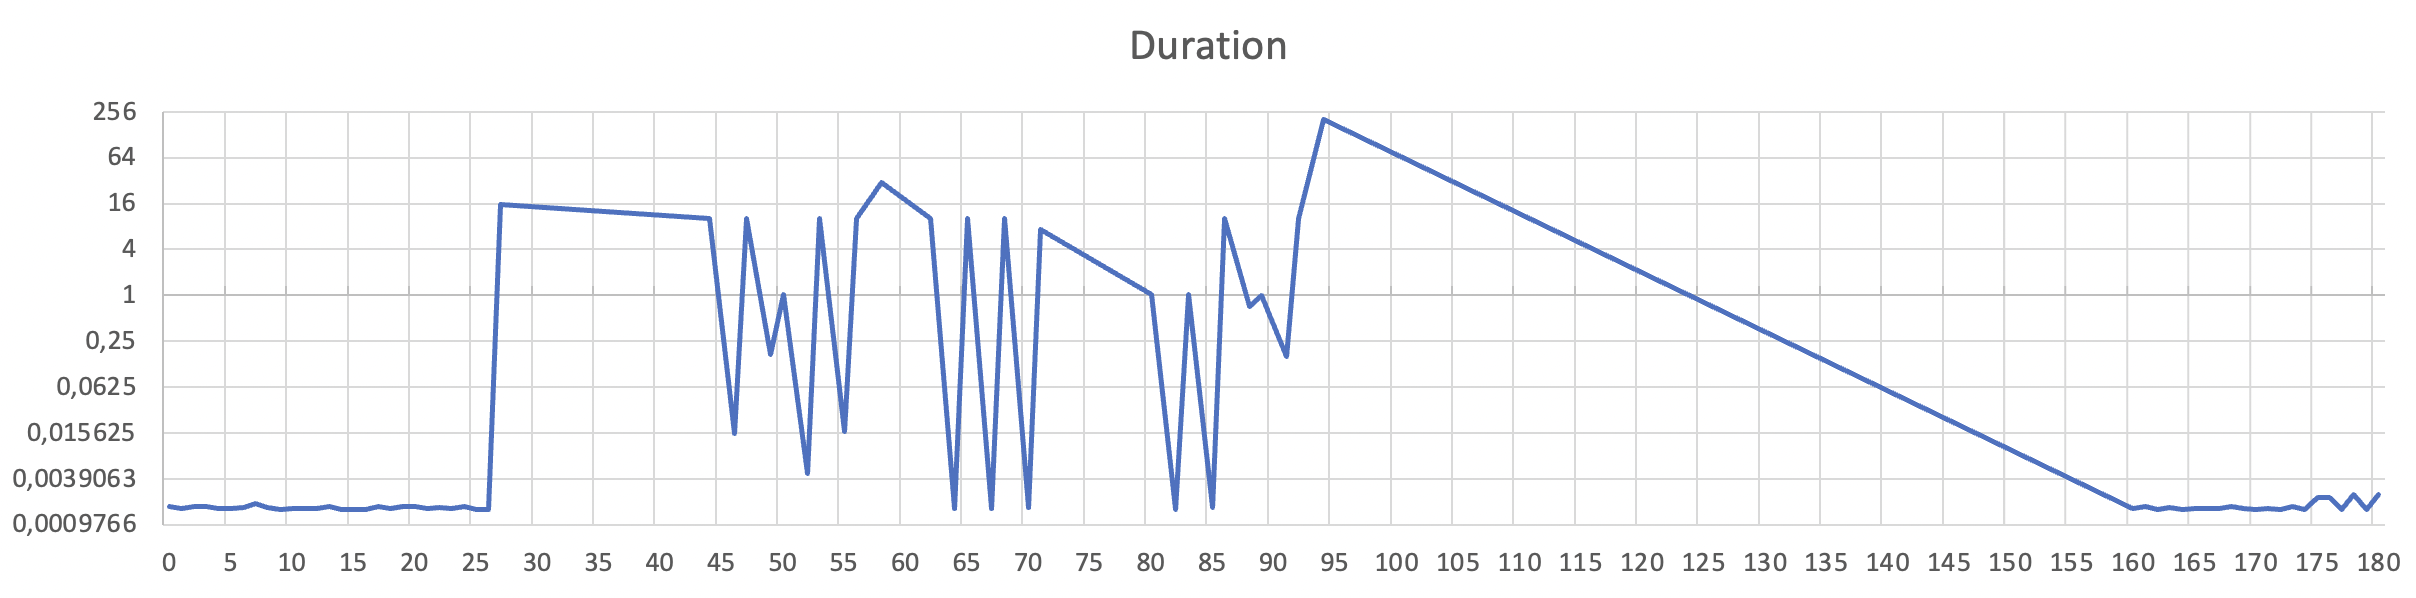
\includegraphics[width=0.8\textwidth]{../drawable/ext2.png}
\end{figure}

\begin{table}[h!]
  \centering
  \begin{tabular}{|l|l|}
    \hline
    Traffic         & Average duration (s)    \\ \hline
    regular traffic & \verb=0.00162= \\ \hline
    with DoS        & \verb=6= \\ \hline
    overall         & \verb=2.2087= \\ \hline
  \end{tabular}
\end{table}

\endgroup
\end{document}